\documentclass[12pt]{article}
\usepackage{amsmath, amssymb, amsfonts, bm, graphicx, geometry, tabularx, booktabs, float, enumitem}
\geometry{margin=1in}

\title{}
\date{}
\author{}

% Uppercase Volume with thicker, higher line
\newcommand{\vol}{\mathord{\text{\ooalign{\hidewidth $V$\hidewidth\cr\kern-0.5pt\raisebox{0.8ex}{\rule[0pt]{1em}{0.5pt}}}}}}

% Lowercase Volume with built-in shifts
\newcommand{\svol}{%
  \mathord{\text{\ooalign{%
    \hfil$v$\hfil\cr
    \hfil\rule[0.6ex]{0.8em}{0.5pt}\hfil
  }}}%
}

\begin{document}
\section*{4-23}
\vspace{-1em}
\begin{center}
    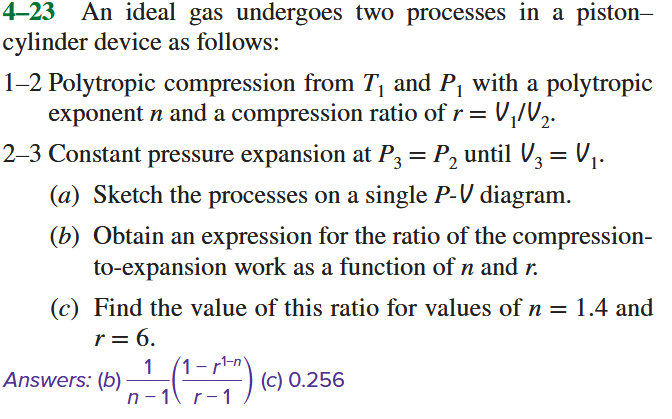
\includegraphics[width=0.5\textwidth]{4-23.png}
\end{center}
\textbf{a)} A polytropic process describes a process where $P\vol^n = \text{constant}$ (this also applies to specific volume $P\svol^n = \text{constant}$ since the mass is a constant). In this case of an ideal gas in a cylinder, $n$ must be positive since we would expect pressure to increase as volume decreases, a negative $n$ would imply the opposite.
\begin{center}
    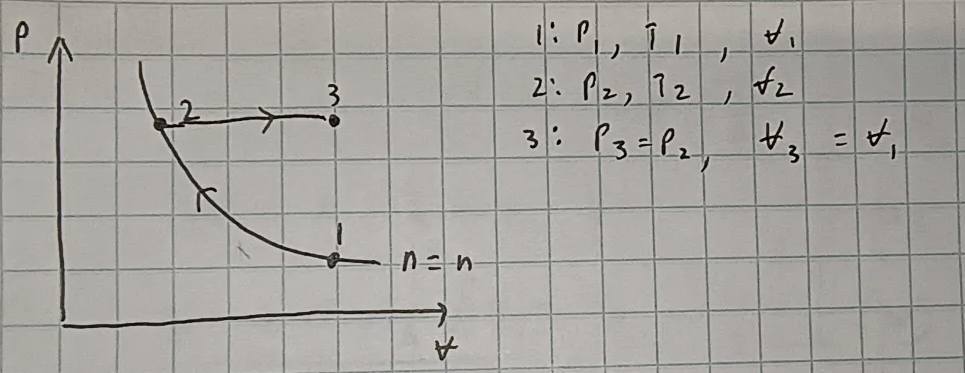
\includegraphics[width=0.5\textwidth]{4-23_1.png}
\end{center}
\textbf{b)} A definition of work done by a system is 
\[W=\int P\,d\vol\]
Where in a polytropic process where $n\neq 1$, 
\[P\vol^n = C \implies P = C\vol^{-n}\]
\[W = \int_{1}^{2} C\vol^{-n} \, d\vol = \boxed{\frac{C}{-n+1} \left( \vol_2^{-n+1} - \vol_1^{-n+1} \right) }\]
For the case where $n=1$,
\[P\vol = C \implies P = C\vol^{-1}\]
\[W = \int_{1}^{2} C\vol^{-1} \, d\vol = \boxed{C \ln\left( \frac{\vol_2}{\vol_1} \right)}\]
Note that for both cases, the constant $C$ is defined by either state 1 or 2 since by definition of a polytropic process, 
$$C = P_1\vol_1^n = P_2\vol_2^n$$
so we can rewrite the work of a polytropic process ($n\neq 1$) as
\[W = C\left(\frac{\vol_2^{-n+1}}{-n+1}\right) - C\left(\frac{\vol_1^{-n+1}}{-n+1}\right) = P_2\vol_2^n\left(\frac{\vol_2^{-n+1}}{-n+1}\right) - P_1\vol_1^n\left(\frac{\vol_1^{-n+1}}{-n+1}\right)\]
\[\boxed{W = \frac{P_2\vol_2 - P_1\vol_1}{-n+1}}\]
Since the problem doesn't specify that the process is isothermal, we will use the $n\neq 1$ case.\\\\
\underline{Compression $1\to2$ (polytropic)}
\[W_\text{comp} = \frac{P_2\vol_2 - P_1\vol_1}{-n+1}\]
\underline{Expansion $2\to3$ (ISOBARIC: constant pressure)}
\[W_\text{exp} = P_2(\vol_3 - \vol_2) = P_2 (\vol_1 - \vol_2)\]
Ratio:
\[\frac{W_\text{comp}}{W_\text{exp}} = \frac{P_2\vol_2 - P_1\vol_1}{(-n+1)(P_2 (\vol_1 - \vol_2))}\]
Rewriting it using the compression ratio
\[r = \frac{\vol_1}{\vol_2} \implies \vol_1 = r\vol_2\]
\[P_1\vol_1^n = P_2\vol_2^n \quad \text{(polytropic)} \implies P_2 = P_1 \left(\frac{\vol_1}{\vol_2}\right)^n = P_1 r^{n}\]
\[\implies \frac{W_\text{comp}}{W_\text{exp}} = \frac{P_1 r^{n}\vol_2 - P_1r\vol_2}{(-n+1)(P_1 r^{n} (r\vol_2 - \vol_2))}\]
Cancelling $P_1\vol_2$ from the numerator and denominator, we get
\[\boxed{\frac{W_\text{comp}}{W_\text{exp}} = \frac{r^{n} - r}{(-n+1)r^{n}(r-1)}}\]
\textbf{c)} Plugging in $n=1.4$ and $r=6$:
\[\frac{W_\text{comp}}{W_\text{exp}} = \frac{6^{1.4} - 6}{(-1.4+1)6^{1.4}(6-1)} \approx \boxed{0.256}\]
\section*{4-44}
\vspace{-1em}
\begin{center}
    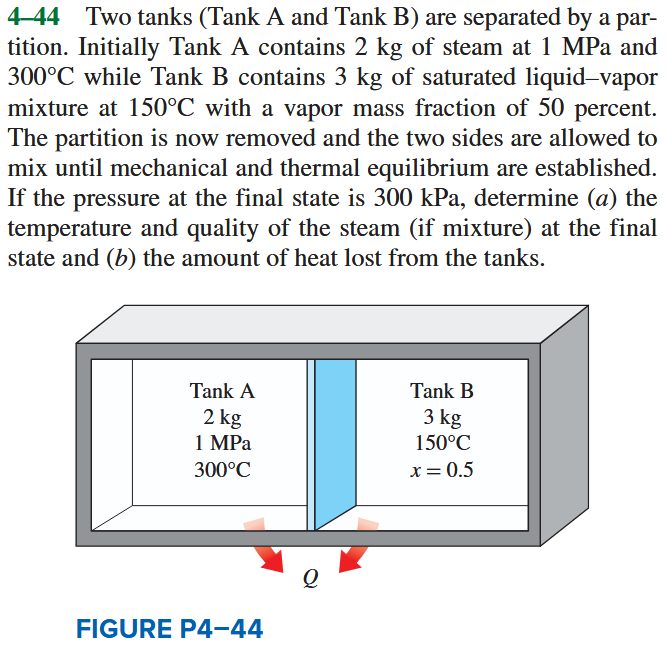
\includegraphics[width=0.6\textwidth]{4-44.png}
\end{center}
Given:
\begin{itemize}
    \item State 1
    \begin{itemize}
        \item Tank A (STEAM): $m_{A1} = 2$ kg, $P_{A1} = 1$ MPa, $T_{A1} = 300^\circ$C
        \item From the superheated water table A-6: $\svol_{A1} =0.25799$ m$^3$/kg, $u_{A1} = 2793.7$ kJ/kg
        \item Tank B (SATURATED MIXTURE): $m_{B1} = 3$ kg, $T_{B1} = 150^\circ$C, $x_{B1} = 0.5$
    \end{itemize}
    \item State 2
    \begin{itemize}
        \item At mechanical and thermal equilibrium
        \item $P_2 = 300$ kPa
    \end{itemize}
    \item The box is rigid and the two sides mix after being initially separated
\end{itemize}
Find: 
\begin{itemize}
    \item The temperature and quality of the steam if it is a mixture at state 2
    \item Amount of heat $Q$ lost during the process
\end{itemize}
Using the quality of B1, we can find the specific volume and internal energy of B1 at $T_{B1} = 150^\circ$C:
\[\svol_{B1} = \svol_f + x_{B1}\svol_{fg}
= [0.001091 + 0.5(0.39248 - 0.001091)] \text{ m}^3/\text{kg}
= 0.19696 \text{ m}^3/\text{kg}
\]
\[u_{B1} = u_f + x_{B1}u_{fg} = [631.66 + 0.5(1927.4)] \text{ kJ/kg} = 1595.36 \text{ kJ/kg}\]
Now state 1 is fully defined.\\\\
\textbf{a)} 
Since the total volume and mass is conserved, we can find the specific volume at state 2:
\[\svol_2 = \frac{m_{A1}\svol_{A1} + m_{B1}\svol_{B1}}{m_{A1} + m_{B1}} = \frac{[2\,\text{kg}][0.25799\,\text{m}^3/\text{kg}] + [3\,\text{kg}][0.19696\,\text{m}^3/\text{kg}]}{2\,\text{kg} + 3\,\text{kg}} = 0.22137 \text{ m}^3/\text{kg}\]
Using this specific volume and the pressure at state 2, we can determine the phase of state 2: SATURATED MIXTURE since $\svol_f < \svol_2 < \svol_g$ at $P_2 = 300$ kPa.\\\\
Now we can find the quality at state 2:
\[x_2 = \frac{\svol_2 - \svol_f}{\svol_{g} - \svol_f} = \frac{0.22137 - 0.001073}{0.60582-0.001073} = \boxed{0.3642}\]
The temperature at state 2 is the saturation temperature at $P_2 = 300$ kPa, which is $\boxed{133.52^\circ\text{C}}$.\\\\
\textbf{b)} Apply the first law for a closed system, keeping in mind that since $\Delta V = 0$ (rigid box), $W=0$:
\[\Delta U = Q - W\]
\[Q = \Delta U = U_2-U_1 = m_2u_2 - (m_{A1}u_{A1} + m_{B1}u_{B1})\]
We can use the quality at state 2 to find the internal energy at state 2:
\[u_2 = u_f + x_2 u_{fg} = 561.11 + 0.3642(1982.1) = 1282.9908 \text{ kJ/kg}\]
Thus,
\[Q = (m_{A1}+m_{B1})u_2 - (m_{A1}u_{A1} + m_{B1}u_{B1})\]
\[= [2+3\,\text{kg}][1282.9908\,\text{kJ/kg}] - [2\,\text{kg}][2793.7\,\text{kJ/kg}] - [3\,\text{kg}][1595.36\,\text{kJ/kg}]\]
\[= \boxed{-3958.526\,\text{kJ}}\]
Note that the negative sign indicates that the system lost heat during the process.
\section*{4-54}
\vspace{-1em}
\begin{minipage}[t]{0.6\textwidth} \vspace{0pt}
\centering
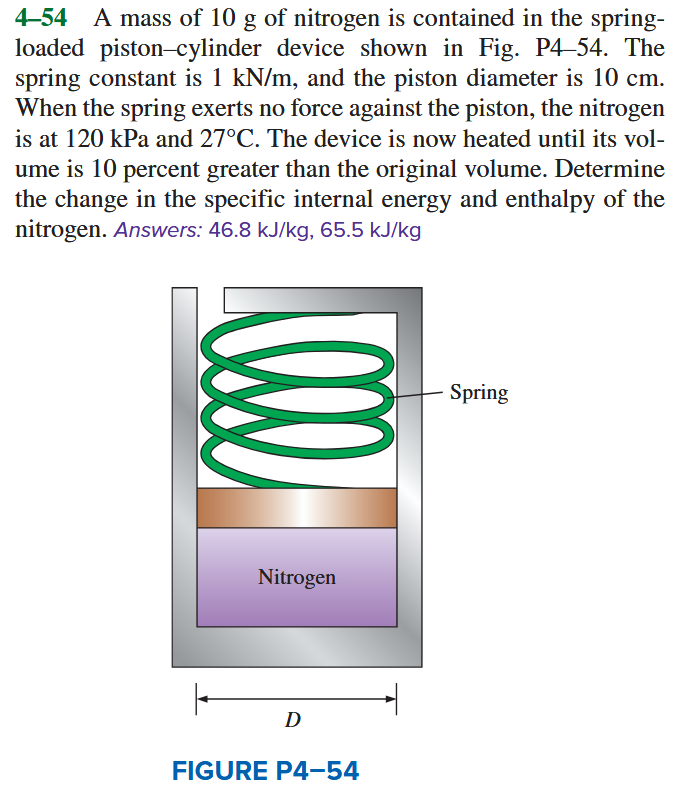
\includegraphics[width=\textwidth]{4-54.png}
\end{minipage}
\hfill
\begin{minipage}[t]{0.4\textwidth} \vspace{0pt}
Given:
\begin{itemize}
    \item Mass of nitrogen gas $m=10 g$
    \item $k=1$ kN/m
    \item $D=10$ cm
    \item State 1: Spring is uncompressed. $P_1 = 120$ kPa, $T_1 = 27^\circ$C, $\vol_1$
    \item State 2: $\vol_2 = 1.1\vol_1$, $P_2$, $T_2$
\end{itemize}
Find: 
\begin{itemize}
    \item Change in specific internal energy $\Delta u$ and specific enthalpy $\Delta h$ from state 1 to state 2
\end{itemize}
\end{minipage}\\\\
Since the nitrogen is a gas, we can use the ideal gas law:
\[P_1\vol_1 = m R T_1\]
\[\vol_1 = \frac{m R T_1}{P_1} = \frac{[0.01\,\text{kg}]\left[0.2968\,\frac{\text{kPa}\cdot\text{m}^3}{\text{kg}\cdot\text{K}}\right][27+273.15\,\text{K}]}{120\,\text{kPa}}=0.007423\,\text{m}^3\]
\[\vol_2 = 1.1\vol_1 = 0.008166\,\text{m}^3\]
Now we can find the displacement of the spring at state 2:
\[\Delta \vol = \frac{\pi}{4} D^2 (x_2 - x_1)\]
\[\implies x_2 = \frac{4\Delta \vol}{\pi D^2} + x_1=\frac{4[0.008166-0.007423\,\text{m}^3]}{\pi (0.1\,\text{m})^2} + 0 = 0.094601\,\text{m}\]
We can find the force exerted by the spring at state 2 and thus the pressure at state 2:
\[P_2 = P_1 + P_{\text{spring}} = P_1 + \frac{kx_2}{\left(\frac{\pi}{4}D^2\right)}\]
\[P_2  = [120\,\text{kPa}] + \frac{[1000\,\text{N/m}][0.094601\,\text{m}]}{\left(\frac{\pi}{4}(0.1\,\text{m})^2\right)} = [120\,\text{kPa}]+[12044.973\,\text{Pa}]\]
\[P_2 = 132.044\,\text{kPa}\]
Now we can find the temperature at state 2 using the ideal gas law again:
\[T_2 = \frac{P_2\vol_2}{m R} = \frac{[132.044\,\text{kPa}][0.008166\,\text{m}^3]}{[0.01\,\text{kg}]\left[0.2968\,\frac{\text{kPa}\cdot\text{m}^3}{\text{kg}\cdot\text{K}}\right]} = 363.298\,\text{K}\]
Finally, we can find the change in specific internal energy and specific enthalpy using the specific heat constants for nitrogen gas:
\[\Delta u = c_v (T_2 - T_1) = [0.743\,\text{kJ/kg}\cdot\text{K}][363.298-300.15\,\text{K}] = \boxed{46.91\,\text{kJ/kg}}\]
\[\Delta h = c_p (T_2 - T_1) = [1.039\,\text{kJ/kg}\cdot\text{K}][363.298-300.15\,\text{K}] = \boxed{65.61\,\text{kJ/kg}}\]
\section*{4-73E}
\vspace{-1em}
\begin{minipage}[t]{0.6\textwidth} \vspace{0pt}
\centering
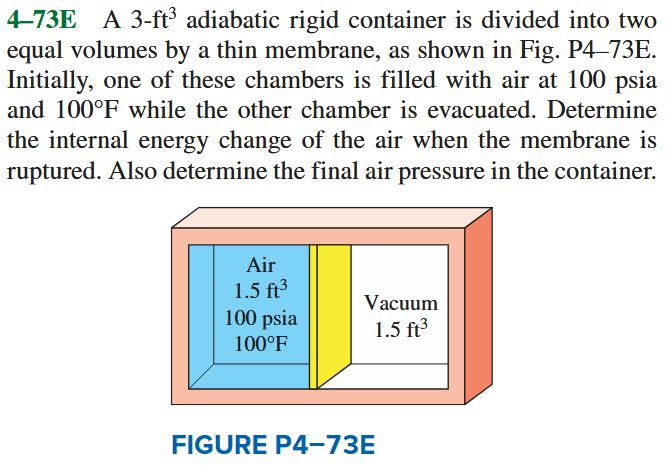
\includegraphics[width=\textwidth]{4-73E.png}
\end{minipage}
\hfill
\begin{minipage}[t]{0.4\textwidth} \vspace{0pt}
Given:
\begin{itemize}
    \item Total volume $\vol_t = 3$ ft$^3$
    \item Adiabatic rigid container ($Q=0$, $W=0$)
    \item State 1: separated evenly into two parts by a partition
    \begin{itemize}
        \item Air: $\vol_{A1} = 1.5$ ft$^3$, $P_{A1} = 100$ psia, $T_{A1} = 100^\circ$F
        \item Vacuum: $\vol_{V1} = 1.5$ ft$^3$, $P_{V1} = 0$ psia
    \end{itemize}
    \item State 2: partition is removed
\end{itemize}
Find: 
\begin{itemize}
    \item Change in internal energy of the air and the final pressure in state 2.
\end{itemize}
\end{minipage}\\\\
Using the first law for a closed system, we can find the change in internal energy of the air:
\[\boxed{\Delta U = Q - W = 0}\]
Since the container is rigid and adiabatic, there is no work done and no heat transfer. Therefore, the internal energy of the air remains constant.\\\\
To find the pressure at state 2, we can use the ideal gas law. But first we need to find the temperature of air at state 2.
\[u_2 - u_1 = c_v (T_2 - T_1) \implies T_2 = T_1 \quad \text{(since $\Delta U=0$)}\]
Thus,
\[T_1 = \frac{P_1 \vol_1}{mR}, \quad T_2 = \frac{P_2 \vol_2}{mR}\]
\[T_1 = T_2 \implies P_1 \vol_1 = P_2 \vol_2\]
\[P_2 = P_1 \frac{\vol_1}{\vol_2}= [100\,\text{psia}] \frac{1.5\,\text{ft}^3}{3\,\text{ft}^3} = \boxed{50\,\text{psia}}\]
\section*{4-138}
\vspace{-1em}
\begin{minipage}[t]{0.6\textwidth} \vspace{0pt}
\centering
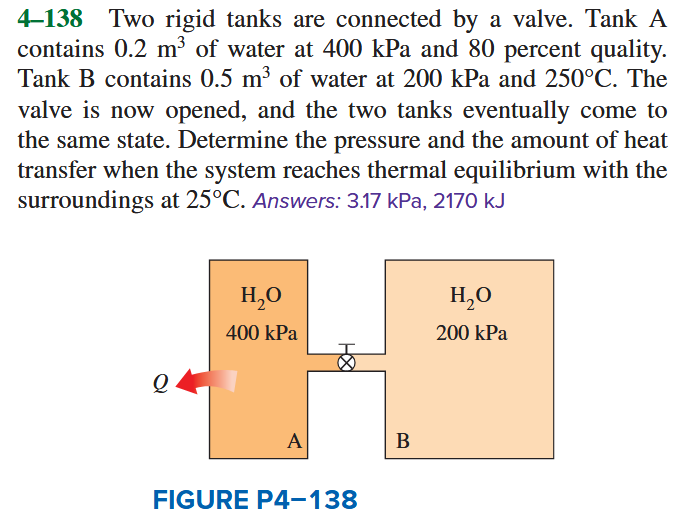
\includegraphics[width=\textwidth]{4-138.png}
\end{minipage}
\hfill
\begin{minipage}[t]{0.4\textwidth} \vspace{0pt}
Given:
\begin{itemize}
    \item Rigid tank ($\Delta \vol =0 \implies W =0$)
    \item State 1:
    \begin{itemize}
        \item A (Water): $\vol_{A1} = 0.2$ m$^3$, $P_{A1} = 400$ kPa, $T_{A1} = ?^\circ$C, $x_{A1} = 0.8$
        \item B (Water): $\vol_{B1} = 0.5$ m$^3$, $P_{B1} = 200$ kPa, $T_{B1} = 250^\circ$C
    \end{itemize}
    \item State 2: At mechanical and thermal equilibrium. $\vol_2$, $P_2$, $T_2=25^\circ$C
\end{itemize}
Find: 
\begin{itemize}
    \item Pressure at state 2 and amount of heat transferred during the process
\end{itemize}
\end{minipage}\\\\
Start by defining state A1. It is a saturated mixture since $x_{A1} = 0.8$. At 400 kPa, the saturation temperature is \underline{$T_{A1} = 143.61^\circ$C}.\\\\
Using the quality, we can also solve for the specific volume and internal energy at state A1:
\[\svol_{A1} = \svol_f + x_{A1}\svol_{fg} = [0.001084 + 0.8(0.46242 - 0.001084)] \text{ m}^3/\text{kg} = \underline{0.37015 \text{ m}^3/\text{kg}}\]
\[u_{A1} = u_f + x_{A1}u_{fg} = [604.22 + 0.8(1948.9)] \text{ kJ/kg} = \underline{2163.34 \text{ kJ/kg}}\]
Next we can define the state B1. At P=200 kPa, $T_{B1}>T_\text{sat}$, so it is a superheated vapor. Looking at the superheated vapor tables we find:
\[\underline{\svol_{B1} = 1.19890 \text{ m}^3/\text{kg}, \quad u_{B1} = 2731.4 \text{ kJ/kg}}\]
With both the total volumes and specific volumes, we can find the masses in state 1:
\[m_{A1} = \frac{\vol_{A1}}{\svol_{A1}} = \frac{0.2}{0.37015} = 0.5403 \text{ kg}\]
\[m_{B1} = \frac{\vol_{B1}}{\svol_{B1}} = \frac{0.5}{1.19890} = 0.4170 \text{ kg}\]
Now lets define state 2:
\[\vol_2 = \vol_{A1} + \vol_{B1} = 0.2 + 0.5 = 0.7 \text{ m}^3\]
\[\implies \svol_2 = \frac{\vol_2}{m_{A1} + m_{B1}} = \frac{0.7}{0.5403 + 0.4170} = 0.7312 \text{ m}^3/\text{kg}\]
At $T_2 = 25^\circ$C, $\svol_2$ is between $\svol_g$ and $\svol_f$, so state 2 is a saturated mixture. Thus, the pressure at state 2 is the saturation pressure at $T_2 = 25^\circ$C, which is $\boxed{3.1698 \text{ kPa}}$.\\\\
Using the quality at state 2, we can find the internal energy at state 2:
\[x_2 = \frac{\svol_2 - \svol_f}{\svol_g - \svol_f} = \frac{0.7312 - 0.001003}{43.340 - 0.001003} = 0.01684\]
\[u_2 = u_f + x_2 u_{fg} = 104.83 + 0.01684(2304.3) = 143.653 \text{ kJ/kg}\]
Finally, we can apply the first law to find the amount of heat transferred during the process:
\[\Delta U = Q - W\]
\[Q = U_2 - U_1  = (m_{A1}+m_{B1})u_2 - (m_{A1}u_{A1} + m_{B1}u_{B1})\]
\[Q = (0.5403 + 0.4170)(143.653) - (0.5403)(2163.34) - (0.4170)(2731.4) = \boxed{-2169.910 \text{ kJ}}\]
\newpage
\section*{4-148}
\vspace{-1em}
\begin{minipage}[t]{0.6\textwidth} \vspace{0pt}
\centering
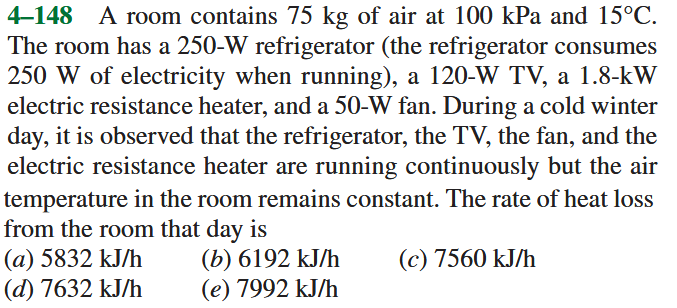
\includegraphics[width=\textwidth]{4-148.png}
\end{minipage}
\hfill
\begin{minipage}[t]{0.4\textwidth} \vspace{0pt}
Given:
\begin{itemize}
    \item $\dot{W}_\text{refrigerator} = 250$ W
    \item $\dot{W}_\text{TV} = 120$ W
    \item $\dot{W}_\text{heater} = 1.8$ W
    \item $\dot{W}_\text{fan} = 50$ W
    \item Refrigerator, TV, fan, and heater are running
\end{itemize}
Find: 
\begin{itemize}
    \item Rate of heat loss in kJ/h if the temp stays constant
\end{itemize}
\end{minipage}\\\\
Since temp is constant, the rate of energy entering must equal the rate of energy leaving. \\\\
Energy in:
\[\dot{W}_\text{refrigerator} + \dot{W}_\text{TV} + \dot{W}_\text{heater} + \dot{W}_\text{fan} = 2220 \text{W}\]
\[\implies \dot{W}_\text{loss} = 2220 \text{W}\]
Convert to kJ/h:
\[\left[2220\, \frac{\text{J}}{\text{s}}\right]\left[\frac{1\text{kJ}}{10^3\text{J}}\right]\left[\frac{3600\text{s}}{1\text{h}}\right] = \boxed{7992 \text{ kJ/h  (e)}}\]
\end{document}